\documentclass[a4paper]{article}
\usepackage{titling}
\usepackage{authblk}
\usepackage{fancyhdr}
\usepackage{hyperref}
\usepackage{rsc}
\usepackage{siunitx}
\usepackage{graphicx}
\usepackage{listings}
\usepackage{color}

\definecolor{dkgreen}{rgb}{0,0.6,0}
\definecolor{gray}{rgb}{0.5,0.5,0.5}
\definecolor{mauve}{rgb}{0.58,0,0.82}

\lstset{frame=tb,
  language=Python,
  aboveskip=3mm,
  belowskip=3mm,
  showstringspaces=false,
  columns=flexible,
  basicstyle={\ttfamily},
  numbers=none,
  numberstyle=\tiny\color{gray},
  keywordstyle=\color{blue},
  commentstyle=\color{dkgreen},
  stringstyle=\color{mauve},
  breaklines=true,
  breakatwhitespace=true,
  tabsize=3
}
\DeclareSIUnit\Fahrenheit{\degree F}

\title{Lecture 1: Introduction to Python}
\author[1]{Dr Benjamin J. Morgan}
\author[1,2]{Dr Andrew R. McCluskey}
\affil[1]{Department of Chemistry, University of Bath, email: b.j.morgan@bath.ac.uk}
\affil[2]{Diamond Light Source, email: andrew.mccluskey@diamond.ac.uk}
\setcounter{Maxaffil}{0}
\renewcommand\Affilfont{\itshape\small}

\pagestyle{fancy}
\fancyhf{}
\rhead{CH40208}
\lhead{\thetitle}
\rfoot{\thepage}

\begin{document}
\maketitle

\section*{Aim}
In this lecture, you will be introduced to Pythonic variable types, basic arithmetic, input and output (I/O) and intrinsic functions.

\section{Introduction}

The aim of this course is to develop skills in the user of computer programming (particularly in the Python programming language), building on the skills learned in the first and second year Computational Chemistry laboratory.
You will then put these skills into practice, using Python to analyse chemical structures and perform quantum mechanical chemical calculations.

The Python programming language is one of the most popular programming languages in the world, ranking third on the TIOBE index (a measure of programming language popularity) in June 2019\cite{tiobe_index}, with the largest rate of change (it is becoming more popular over time).
Additionally, it is probably the most popular programming language used in the chemical sciences.
Recently, it was suggested that more than \SI{7}{\percent} of all academic papers published in 2018 made mention of the Python (Figure~\ref{fig:pic}) \cite{arm_pycon}.
%
\begin{figure}[t]
\centering
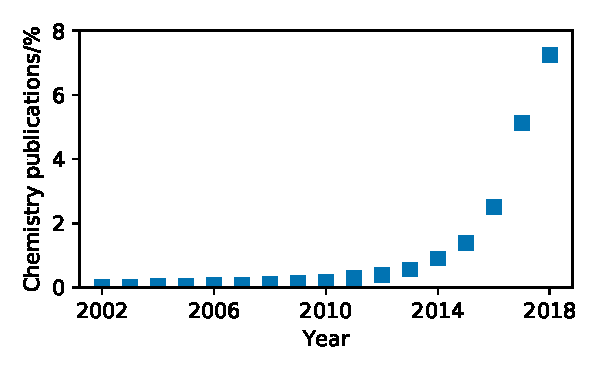
\includegraphics{chem_data_py}
\label{fig:pic}
\caption{The percentage of ``chemistry'' publications that also mention ``python'', determined from the numbers of matching Google Scholar results.}
\end{figure}
%

Python was first released in 1991, with one of the main design philosophies of the language being code readability.
This readability is one of the driving factors to its adoption, along with some of the concepts introduced in this course, such as dynamical typing and powerful libraries like NumPy and Matplotlib.
Since the early 1990s there have been three major versions of Python, with the most recent (and the focus of this course) being Python 3.
Python 2 is still commonly found online and in libraries, however it is due to ``retire'' at the end of this year (check out \url{https://pythonclock.org} for a live countdown).
Therefore, many packages are now dropping support for Python 2 and most practitioners would suggest new learners to start with Python 3.

\subsection{Books}

While this course is self-contained, the following books are particularly useful for those interested in learning more about Python:
\begin{itemize}
	\item J. Vanderplas, \emph{Python Data Science Handbook}, O'Reilly Media, Sebestopol, 2016. This book is available as a free e-book at: \url{https://jakevdp.github.io/PythonDataScienceHandbook/}.
\end{itemize}

\section{Variable types}

It is the case in many programming languages that \emph{variables} can be assigned, a variable is a container used to store some data.
It is possible to assign a variable as shown below,
\begin{lstlisting}
# Variable assignment

banana = 1.
\end{lstlisting}
Not all variables are the same, and therefore variables may have different \emph{types}, where different operations are possible depending on the type.
Some examples of variable types that are present in Python include:
\begin{itemize}
	\item{\textbf{Integers} (\texttt{int}) -- these are whole numbers ($1$, $2$, $0$, $-3$, etc.); there is no decimal point, and they can be positive, negative, or zero.}
	\item{\textbf{Floats} (\texttt{float}) -- these are all \emph{real} numbers ($1.0$, $3.14$, $0.0$, $6.28$, etc.); any values that can be described using a decimal point.}
	\item{\textbf{Complex} (\texttt{complex}) -- complex numbers should be familiar from mathematics, where they are typically written as $2+1i$, however in Python the $i$ is replaced with a \texttt{j}, so $2+1i$ becomes \texttt{2+1j}.}
	\item{\textbf{String} (\texttt{str}) -- a string is a textual variable such as a word or a sentence. These are written between single or double inverted commas, \texttt{`like this'} or \texttt{"this"}.}
	\item{\textbf{Boolean} (\text{bool}) -- named for George Boole, who first defined an algebraic logic system in the 19th century, a Boolean is a \emph{logical} variable type that may hold one of two values, either \texttt{True} or \texttt{False}.}
\end{itemize}
The type of a given variable can be determined with the following command,
\begin{lstlisting}
# Type determination

type(banana)
\end{lstlisting}
This function will return the type of the variable given as an \emph{argument}.

\vspace{\baselineskip}
\begin{center}
	\noindent\fbox{%
	    \begin{minipage}{0.9\textwidth}%
	        \vspace{0.15\baselineskip}
			\subsubsection*{Exercise}
	        \begin{itemize}
	        	\item{Experiment with the different variable types and see if you can assign an example variable for each of the five outlined above.}
	        	\item{Determine the type of each of the following:}
	        	\begin{enumerate}
	        		\item{\texttt{greeting = "Hello World!"}}
	        		\item{\texttt{pi = 3.1415}}
	        		\item{\texttt{life = 42}}
	        	\end{enumerate}
	        	\item{Consider the type difference between \texttt{1}, \texttt{1.}, and \texttt{1.0} as interperated by Python.}
	        \end{itemize}
	    \end{minipage}
	}
\end{center}

\section{Variable assignment}

It was mentioned above that a variable may be assiged with the following syntax,
\begin{lstlisting}
# Variable declaration

banana = 1.
\end{lstlisting}
This establishes a name (\texttt{banana}) for some location in the computer memory, and places a value (\texttt{1.}) into that location.
Once a variable has been assigned, it can be used in other parts of the code.
For example consider,
\begin{lstlisting}
# Reuse banana

apple = 5. + banana
\end{lstlisting}
Above, we have reused the banana variable assigned previously to create a new variable, \texttt{apple}.
\vspace{\baselineskip}
\begin{center}
	\noindent\fbox{%
	    \begin{minipage}{0.9\textwidth}%
	        \vspace{0.15\baselineskip}
			\subsubsection*{Exercise}
	        \begin{itemize}
	        	\item{Investigate the effect of changing the value of \texttt{banana}, after the variable \texttt{apple} has been defined.}
	        \end{itemize}
	    \end{minipage}
	}
\end{center}

\section{Computer arithmetic}

Python is able to basic mathematical operations natively (without the need for additional libraries to be loaded), some of these are shown in Table~\ref{tab:ops}.
\begin{table}[h]
	\centering
	\caption{The Python syntax for some basic mathematical operations.}
	\label{tab:ops}
	\begin{tabular}{c c c}
		\hline
		Operation & Mathematical notation & Pythonic notation \\
		\hline
		Addition & $a + b$ & \texttt{a + b} \\
		Subtraction & $a - b$ & \texttt{a - b} \\
		Multiplication & $a \times b$ & \texttt{a * b} \\
		Division & $a \div b$ & \texttt{a / b} \\
		Exponent & $a^b$ & \texttt{a ** b} \\
		\hline
	\end{tabular}
\end{table}

Using these basic tools alone, it is possible to use a Jupyter Notebook as a rudimentary calculator.

\subsection{Order of operations}

A single line of code can include many of the arithmetic operations outlined above, therefore it is necessary to establish a hierarchy, also known as the \emph{order of operations}.
Python follows the order of operations that should be familiar from mathematics, you may know this as BODMAS:
\begin{enumerate}
	\item{\textbf{B}rackets}
	\item{\textbf{O}rder}
	\item{\textbf{D}ivide}
	\item{\textbf{M}ultiply}
	\item{\textbf{A}ddition}
	\item{\textbf{S}ubtraction}
\end{enumerate}
\vspace{\baselineskip}
\begin{center}
	\noindent\fbox{%
		\begin{minipage}{0.9\textwidth}%
			\vspace{0.15\baselineskip}
			\subsubsection{Exercise}
			\begin{itemize}
				\item{Without using the computer, and following the order of operations defined above, calculate the following:}
				\begin{enumerate}
					\item{$24 \div (10 + 2)$}
					\item{$5 + 16 \div 2 \times 3$}
					\item{$(32 \div (6 + 2))^2$}
				\end{enumerate}
				\item{Now check your answers are correct using the computer.}
			\end{itemize}
		\end{minipage}
	}
\end{center}

\subsection{Mixed mode operations}

When the two operands are of the same type, the result of an arithmetic operation will also be of that type.
However, the operation is on two operands of different types it is necessary to modify one of them before the operation is performed.
For example, in the code below, an \texttt{int} is divided by a \texttt{float} and the type of the result will be a \texttt{float},
\begin{lstlisting}
# Divide an int by a float

mixed_type = 2 / 4.0

type(mixed_type)
\end{lstlisting}
This is because the \texttt{2} is converted to a \texttt{float}, so the operation becomes effectively \texttt{2.0 / 4.0}.

As of Python 3, if one \texttt{int} is divided by another \texttt{int} then both are converted to a \texttt{float}, meaning that, in the code below, the variable \texttt{both\_int} will be a \texttt{float} with a value of \texttt{0.5},
\begin{lstlisting}
# Divide an int by a float

both_int = 2 / 4

type(both_int)
\end{lstlisting}
In Python 2, this would have returned an \texttt{int} with a value of \texttt{0}, however, with Python 3 the ``floor division'' operator (\texttt{//}) must be used to achieve this result,
\begin{lstlisting}
# Divide an int by a float

floor_division = 2 // 4

type(floor_division)
\end{lstlisting}

\section{Print and input (I/O) methods}

Until now, you have been using the Jupyter Notebook to ``print'' the information.
You may have noticed that the result of the final line in a given cell will be printed below it.
However, if you would like to get information from a different part of a cell (or from within a larger program as we will see in later weeks), it is necessary to be able to print from the code.
This is where the \emph{print statement} comes in, in Python this looks like this,
\begin{lstlisting}
# Print Hello World!

print("Hello World!")
\end{lstlisting}
This should output the string \texttt{"Hello World!"} when the cell is run (some of you may be aware that printing Hello World! is considered a right of passage in programming and is often the first thing someone will do when learning a new programming language).

Any of the types discussed above may be printed with the print statement, additionally it is also possible to use the print statement to insert numerical values into a string.
We can even prescribe how the number is written, for example in the code below the information between the curly brackets tells the Python \emph{interpreter} that the floating point number (\texttt{f}) should be written with two (\texttt{2}) numbers following the decimal point (\texttt{.}).
\begin{lstlisting}
# More interesting printing

pi = 3.1415

print("pi to 4 decimal places is {} exactly!".format(pi))
print("pi to 2 decimal places is {:.2f} exactly!".format(pi))
\end{lstlisting}

In addition to printing, it is also possible to read information from the user.
This is achieved using the \texttt{input} function, which will read the information given by the user as a string and store is in the defined variable.
The code below will test out the \texttt{input} and \texttt{print} functions,
\begin{lstlisting}
# Who am I?

my_name = input("What is your name?")

print(my_name)
\end{lstlisting}

\section{Problem}

The final exercise of this week is to, in a single Jupyter Notebook cell, write some code that would allow a user to input a temperature in Fahrenheit and convert this to Celsius.
For reference,
\begin{equation}
	T (\si{\celsius}) = \frac{5 ( T(\si{\Fahrenheit}) - 32)}{9}.
\end{equation}
You should consider how this may be broken down into \emph{four} simple steps, write these steps out as an \emph{algorithm} and then write your code from this algorithm.
If you manage to complete this write another cell to convert from Fahrenheit to Kelvin.

\bibliographystyle{rsc}
\bibliography{handout_1}

\end{document}
